\section[ЛР №3. Модель обслуживания PaaS, Heroku]{Лабораторная работа №3. \\
Модель обслуживания PaaS на примере деплоя приложения в Heroku}

\textbf{Цель работы:} ознакомиться с моделью гибкой (agile) разработки программного обеспечения, развернуть приложение на Heroku, ознакомиться с системой контроля версий Git.

\subsection{Краткие сведения о методологиях разработки ПО}
За время существования информационных технологий создавались и изменялись подходы к построению информационных систем.
Первой моделью информационной системы была монолитная архитектура.
В данной модели на одном компьютере работали и приложения и база данных (БД), а пользователи сидели у <<тонких>> терминалов которые отображали информацию с компьютера.
У данной архитектуры было большое количество недостатков, поэтому впоследствии ее сменила более перспективная клиент-серверная архитектура.
В этом случае на компьютере располагался выделенный сервер баз данных, а пользователи с <<толстых клиентов>> разгружали сервер БД.

Затем появилась более современная многоуровневая архитектура, у которой логика приложений вынесена на отдельный компьютер, который называется сервер приложений, а пользователи работали на <<тонких>> клиентах через веб-браузеры.
В современном информационном мире большинство приложений выполнено именно в многоуровневой архитектуре.
Она подразумевает развертывание всей ИТ-инфраструктуры на территории заказчика.

\begin{figure}[ht]
    \centering
	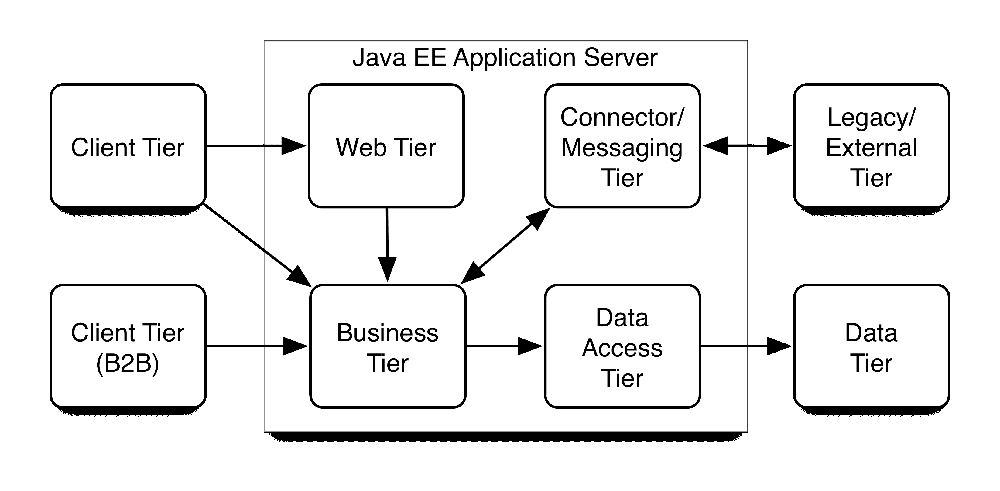
\includegraphics[width=\linewidth]{jee}
	\caption{Пример многоуровневой архитектуры}\label{pic:jee}
\end{figure}

Организация процесса разработки ПО также претерпела много изменений с течением времени.
Одна из самых старых методологий "--- каскадная (водопадная), подразумевает последовательное прохождение стадий, каждая из которых должна завершиться полностью до начала следующей.
В этой модели легко управлять проектом.
Благодаря ее жесткости, разработка проходит быстро, стоимость и срок заранее определены.

В <<гибкой>> (Agile) методологии разработки после каждой итерации заказчик может наблюдать результат и понимать, удовлетворяет он его или нет.
Это одно из преимуществ гибкой модели.
К ее недостаткам относят то, что из-за отсутствия конкретных формулировок результатов сложно оценить трудозатраты и стоимость, требуемые на разработку.
Экстремальное программирование (XP) является одним из наиболее известных применений гибкой модели на практике.

\begin{figure}[ht]
    \centering
	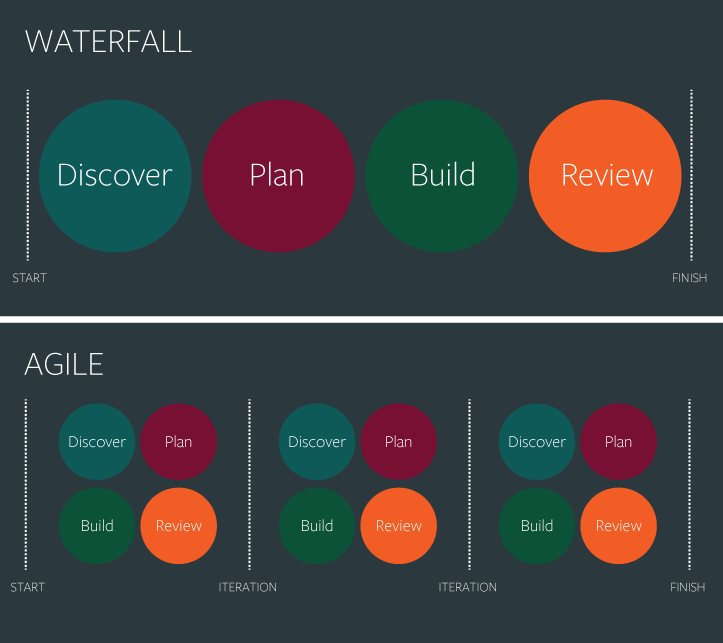
\includegraphics[width=\linewidth]{agile-waterfall}
	\caption{Каскадная и Agile-методологии}\label{pic:agile-waterfall}
\end{figure}

В последнее время все большую популярность приобретает именно Agile-методология, в которой необходимо на каждой итерации разработки проводить развертку новой версии ПО, гораздо удобнее это делать с помощью PaaS-решений, таких как Heroku.

Heroku является облачной PaaS-платформой, поддерживающей ряд языков программирования, таких как Java, Node.js, Scala, Clojure, Python и PHP.
В Heroku можно легко развертывать (деплоить) проекты, не беспокоясь о развертывании собственной инфраструктуры для одного приложения.
Приложения, работающие на Heroku, используют также DNS-сервер Heroku.
Для каждого приложения выделяется несколько независимых виртуальных процессов, которые называются <<dynos>>.
Они распределены по специальной виртуальной сетке <<dynos grid>>, которая состоит из нескольких серверов.
Heroku также поддерживает систему контроля версий Git, а также подключение к аккаунту GitHub.

\subsection{Порядок выполнения работы}

В качестве сервера может использоваться виртуальная машина с установленным дистрибутивом Debian, ранее установленная в лабораторной работе №1.
Виртуальная машина должна иметь доступ в сеть Интернет для скачивания нужных пакетов и работы с Heroku.

\begin{enumerate}
    \item Зарегистрироваться в Heroku\footnote{Пример работы с Heroku представлен в прил.~\ref{pril:e}};
    \item Создать тестовое приложение на языке Python;
    \item Задеплоить приложение на Heroku;
    \item Внести изменения в исходный код приложения и снова задеплоить приложение;
    \item Ознакомиться с дополнительными возможностями Heroku и Git.
\end{enumerate}

\subsection{Контрольные вопросы}
\begin{enumerate}
    \item Почему методология гибкой разработки ПО становится все более популярной?
    \item В чем преимущество использования PaaS-решений по сравнению с IaaS для развертывания своего ПО?
    \item Для чего необходима команда commit в Git?
    \item В чем преимущество использования Heroku по сравнению с деплоем в локальном окружении?
\end{enumerate}

\clearpage
